\section{Auditable memory tails: what a source contract can justify}
\label{sec:audited_tails}
The v0.4 observation experiment leaves a consequential gap: a short response record cannot validate the minimum learning rate that makes its upper bound finite. We now separate an \emph{implementation-conditioned tail claim}, an \emph{observable linear-gain claim}, and a \emph{finite-horizon operational-risk claim}. They have different assumptions and targets. A successful result for one is not silently promoted to the others. The following studies are new to version~0.5; the earlier studies and their adverse findings remain unchanged.

\subsection{A complete channel inventory, not a guessed rate floor}
The audited experimental class has the public update rule
\begin{equation}
 m_{i,t+1}=(1-\eta_i)m_{i,t}+\eta_i x_t,\qquad
 x_{t+1}=a x_t+\sum_i q_i m_{i,t}+\lambda u_t+w_{t+1},
 \label{eq:audited_recursion}
\end{equation}
with $m_{i,0}=x_0=0$, $0\le a<1$, $q_i\ge0$, $\sum_iq_i\le Q_{\max}$, and public $\eta_i\in[\eta_0,1]$. Here $Q_{\max}=1$ is enforced by input validation in the released linear source. The rates, reset, update timing, and absence of other feedback channels are architectural disclosures; they are not estimated from price records. The actual $q_i$, $a$, and $\lambda$ are withheld from the estimator.

The release includes a machine-readable contract with source digest, public rates, zero-reset declaration, observation specification and allowed execution regime. Unit tests reject declared changes to the reset, source digest, observation type, or execution regime. In the experiment the contract is issued from the actual public simulation configuration, and the source is available for inspection. This justifies the restriction \emph{within that controlled implementation}, not in an arbitrary proprietary market.

A digest establishes file identity, not completeness, truthful reporting, or secure runtime attestation. A deliberately self-issued contract containing false rates still passes a syntax-and-digest check. This failure is included in the release. An outside application needs authenticated configuration and an independently inspected inventory of every feedback-relevant channel. A manifest alone is not a safety certificate. In particular, a signal-memory reset does not reset account equity, outstanding positions, leverage rules, or other agents.

\begin{proposition}[Implementation-conditioned tail envelope]
\label{prop:audited_tail}
For the nonnegative memory kernel $k_j=\sum_iq_i\eta_i(1-\eta_i)^j$ generated by \cref{eq:audited_recursion}, a complete valid contract implies
\begin{equation}
 R_H:=\sum_{j=H}^{\infty}k_j
 =\sum_iq_i(1-\eta_i)^H
 \le Q_{\max}(1-\eta_0)^H.
 \label{eq:audited_tail}
\end{equation}
More generally, for $k_j=CA^jB$, induced-norm bounds $\norm{A}\le r<1$, $\norm{B}\le b$ and $\norm{C}\le c$ imply
$\sum_{j=H}^{\infty}\norm{k_j}\le bc\,r^H/(1-r)$.
\end{proposition}
\begin{proof}
Sum each geometric series to obtain the equality in \cref{eq:audited_tail}; nonnegativity and $1-\eta_i\le1-\eta_0$ give the bound. For the second statement, submultiplicativity gives $\norm{CA^jB}\le cb r^j$; summing proves the claim. These are standard geometric-series and induced-norm arguments, not new general stability theorems.
\end{proof}

For $Q_{\max}=1$ and $H=64$, the envelopes at $\eta_0=0.002,0.02,0.1$ are respectively $0.879741$, $0.274454$, and $0.001179$. The slowest contract therefore still permits a large unseen tail. A verified small rate is not equivalent to a useful small tail. If an additional relevant inventory coordinate has unit persistence, the premise $r<1$ for the complete hidden subsystem is unavailable; a contract for the memory module cannot fill that gap.

\subsection{Why the earlier impossibility results still matter}
The exact and noisy counterexamples in Sections~\ref{sec:integrated_hidden}--\ref{sec:integrated_audit} are not contradicted. They concern a less informative observation class. Disclosing the true update architecture and guaranteeing a reset changes the compatible model set. That disclosure has an institutional cost and is not available merely because prices are observed accurately. The distinction between information sufficient for a property and information sufficient for full model recovery is established in data-informativity research \citep{vanwaarde2020}; positive side-information is likewise an existing identification tool \citep{khosravi2025}. Our contribution here is an explicit, executable conditional contract and a documented failure when its scope is misrepresented.

\section{Budgeted inference from audited public dynamics}
\label{sec:budgeted_audit}
\subsection{One terminal innovation per independent episode}
Given public rates, exact midprice deviations and a verified reset, the estimator reconstructs
\begin{equation}
 m_{i,T-1}=\eta_i\sum_{s=1}^{T-2}(1-\eta_i)^{T-2-s}x_s
 \label{eq:observable_memory}
\end{equation}
from prices alone. It never reads the simulator's stored memory. Assume $u_{T-1}=0$. Each independent episode contributes exactly one regression row,
\begin{equation}
 Y_j=x_{j,T_j},\qquad
 X_j=(1,x_{j,T_j-1},m_{j,1,T_j-1},\ldots,m_{j,d,T_j-1}),
 \quad Y_j=X_j\beta+w_{j,T_j},
 \label{eq:terminal_regression}
\end{equation}
where $\beta=(\mu,a,q_1,\ldots,q_d)^\top$ and the intercept accommodates a common mean innovation. The endpoint $T_j$ is fixed or randomly assigned \emph{before} observing that episode. It is not selected after a favorable price movement.

\begin{proposition}[Conditional terminal-row confidence; classical regression]
\label{prop:terminal_confidence}
Suppose episodes are independent, the innovations $w_{j,T_j}$ are independent Gaussian variables with common unknown variance, and each is independent of all pre-terminal regressors and preassigned endpoints. If $X$ has full column rank $p<n$, then for a fixed contrast $v$,
\begin{equation}
 \frac{v^\top\widehat\beta-v^\top\beta}
 {\widehat\sigma\sqrt{v^\top(X^\top X)^{-1}v}}
 \sim t_{n-p}\quad\hbox{conditional on }X.
 \label{eq:terminal_pivot}
\end{equation}
In particular $v=(0,1,1,\ldots,1)$ gives a confidence interval for
$A_{\mathrm{fb}}=a+\sum_iq_i$, whose threshold is one in the maintained positive linear class.
\end{proposition}
\begin{proof}
Conditional on $X$, the last innovations are an independent spherical Gaussian vector. The least-squares projection and orthogonal residual projection are independent. The contrast is Gaussian with variance $\sigma^2v^\top(X^\top X)^{-1}v$, and the residual sum of squares divided by $\sigma^2$ is $\chi^2_{n-p}$. Their ratio gives \cref{eq:terminal_pivot}. No independence claim is made for multiple successive transitions from the same episode; treating those as independent rows would invalidate this proof.
\end{proof}

This is ordinary regression under an explicitly auditable experimental design, not a new superior estimator. Unknown-rate v0.4 recurrence bounds and the present estimator do not receive the same information. The present price observations are exact midquotes rather than the additional sensor-error observations in v0.4. Its initial memory is reset to zero. Consequently, improvement over v0.4 cannot be attributed solely to statistical efficiency.

\subsection{Primary budget experiment and negative results}
The primary v0.5 panel uses the same twelve $(G,\eta_{\mathrm{slow}})$ combinations as v0.4: $G\in\{0.7,0.95,1.05,1.3\}$, $\eta_{\mathrm{slow}}\in\{0.002,0.02,0.1\}$, a fast rate of $0.5$, $a=0.4$, $\lambda=0.02$, and $q=0.6G(0.6,0.4)$. Gaussian innovation standard deviation is $0.002$ dollars. Gains and innovations are not inputs to inference. There are $n\in\{32,128,512\}$ independent episodes, lengths $T\in\{16,64\}$, two probe designs, and twenty replicate panels per cell: 2,880 panels and 645,120 episode trajectories.

The two designs have four shares of within-window gross probe volume: an initial signed four-share impulse or eight half-share orders in four round trips. They do \emph{not} have equal squared input energy or residual inventory. The impulse has energy 16 share-squared and holds four shares at its endpoint; the round trips have energy 2 and return flat, with peak absolute inventory at most half a share. Unwinding the impulse after observation requires another four shares of volume. These economic differences are reported rather than hidden behind a claim of ``equal budget.'' Input design under amplitude and power constraints is established research \citep{manchester2010}; neither pattern is claimed optimal.

Across primary panels, 2,758 of 2,880 gain intervals cover the true gain (95.76\%); 745 give definite labels and twenty give wrong confident labels. Those are empirical frequencies under per-panel 95\% intervals, not simultaneous study-wide coverage. At $T=64,n=128$, the impulse resolves 86/240 panels, versus 46/240 for the round trips. At $n=512$, those counts are 158/240 and 80/240. The round-trip alternative fails as a general accuracy improvement. Its smaller position exposure is a separate property, not proof of equivalent informativeness.

\subsection{Held-out endpoint diversification: useful at small budgets, not uniformly}
After the primary experiment, a small pilot suggested varying the observation endpoint instead of redistributing the order volume. A fresh-seed follow-up was specified before its execution. Both arms use the same initial four-share impulse and the same audited rates. One arm records 64 transitions per episode. The other assigns equal numbers of episodes to 8, 16, 32 and 64 transitions, shuffled before inspecting prices. Its average record is 30 transitions, with the same maximum of 64. Both arms would require the same four-share post-observation unwind, outside the measurement law.

Each paired dataset is simulated to length 64, but the diversified estimator is given only the assigned prefixes; a test alters all later prices and verifies unchanged inference. There are 720 fresh panel datasets (161,280 episodes), each evaluated in both arms, yielding 1,440 decision rows. This is post-primary held-out confirmation, not external preregistration. The contrasts, model grid and new seeds are released.

\begin{table}[htbp]
\centering\small
\caption{Held-out endpoint comparison. Each entry uses 240 panels. Wrong calls are included in, not removed from, the definite-call count.}
\label{tab:endpoint_results}
\begin{tabular}{r r r r r}
\toprule
Episodes & Fixed 64: definite & Wrong & Diversified: definite & Wrong\\
\midrule
32 & 26 (10.83\%) & 0 & 75 (31.25\%) & 2\\
128 & 86 (35.83\%) & 0 & 112 (46.67\%) & 1\\
512 & 159 (66.25\%) & 1 & 144 (60.00\%) & 0\\
\bottomrule
\end{tabular}
\end{table}

At 32 episodes, 56 previously unresolved paired cases become definite and seven go the opposite way: 49 net additional decisions. At 128, the corresponding counts are 42 and sixteen. At 512, diversification loses fifteen decisions net. Thus the result is a budget-dependent trade-off, not a uniformly dominating detector. The release includes descriptive paired tests; pooling heterogeneous model settings is not a claim of universal statistical superiority. In the original fixed-64 primary experiment, the slowest rate resolves only 4/80 panels at 128 episodes and 15/80 at 512. Architectural disclosure does not remove low signal-to-noise limitations.

\begin{figure}[htbp]
\centering
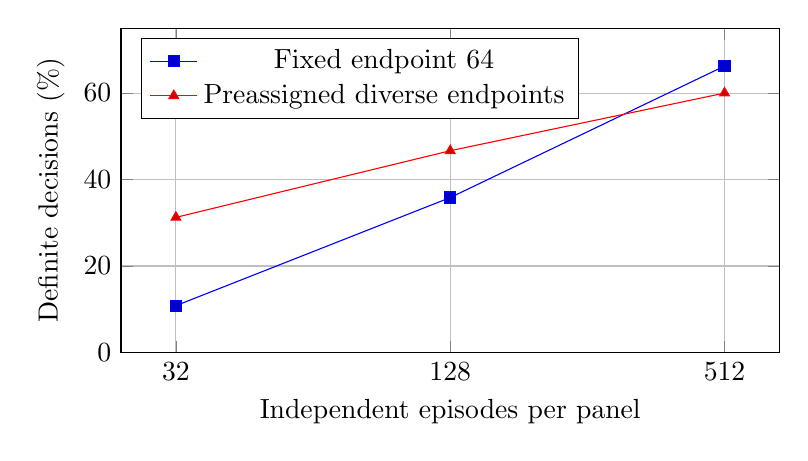
\begin{tikzpicture}
\begin{axis}[width=.82\textwidth,height=5.7cm,xmode=log,log basis x=2,
 xtick={32,128,512},xticklabels={32,128,512},ymin=0,ymax=75,
 xlabel={Independent episodes per panel},ylabel={Definite decisions (\%)},
 legend pos=north west,grid=major]
\addplot+[mark=square*] coordinates {(32,10.8333) (128,35.8333) (512,66.25)};
\addlegendentry{Fixed endpoint 64}
\addplot+[mark=triangle*] coordinates {(32,31.25) (128,46.6667) (512,60)};
\addlegendentry{Preassigned diverse endpoints}
\end{axis}
\end{tikzpicture}
\caption{Observed decision rates on the held-out paired panel. The crossing is retained: a useful low-budget change does not improve every budget. Error counts appear in \cref{tab:endpoint_results}.}
\label{fig:endpoint_tradeoff}
\end{figure}

\subsection{A measured tail interval under the stronger audit}
When rates are genuinely public, the unseen-tail mass in \cref{eq:audited_tail} is itself a linear contrast of $\beta$. Use
$v_H=(0,0,(1-\eta_1)^H,\ldots,(1-\eta_d)^H)$ in \cref{eq:terminal_pivot}. Intersect its interval with $[0,Q_{\max}(1-\eta_0)^H]$. An empty intersection is a model conflict, not an interval silently clipped into feasibility. Splitting $\alpha=0.05$ equally between the gain and tail gives at least 95\% joint coverage per panel by a union bound.

This analysis reuses the primary observations; it creates no additional independent market data. For $H=64$, the joint event holds in 2,796/2,880 panels (97.08\%). There are nine model conflicts. At a fixed observation length of 64, the statistical upper bounds below are medians across eighty panels; they are not worst-case bounds for every episode or every institution.
\begin{table}[htbp]
\centering\small
\caption{Audited tail envelope and median measured upper endpoint for the four-share impulse. Each statistical interval allocates 2.5\% error to the tail.}
\begin{tabular}{r r r r}
\toprule
Minimum rate & Analytic envelope & 128 episodes & 512 episodes\\
\midrule
0.002 & 0.879741 & 0.788458 & 0.490520\\
0.020 & 0.274454 & 0.136919 & 0.103451\\
0.100 & 0.001179 & 0.000674 & 0.000451\\
\bottomrule
\end{tabular}
\end{table}

\subsection{Assumption violations remain visible}
Five eighty-panel controls evaluate deliberately ungated inference. Omitting a slow state produces eighty false stable classifications in eighty panels. Omitting a positive inventory-feedback channel produces three false stable classifications in eighty panels. Noisy regressors and a violated reset produce no wrong labels in their particular runs, but their calibration theorem is still unavailable; absence of observed errors is not proof of robustness. The valid control produces eighty correct unstable classifications. All outcomes, including unhelpful and non-failing controls, are retained. A fit cannot authenticate the architecture that made its confidence statement valid.

\section{Binding financial constraints and a different risk target}
\label{sec:binding_finance}
\subsection{A funded transaction model, not just a ledger}
Version~0.4 records trades but does not impose binding capital constraints. The new financial experiment contains two memory traders, a fundamentalist, a background-flow trader, a probe account and a dealer. Let $C_i$, $I_i$, $P$ and $E_i=C_i+I_iP$ denote cash, shares, midpoint and marked equity. A trade $v_i$ executes at the current midpoint plus a half-spread $s$ paid in the direction of the trade:
\begin{equation}
 C_i'=C_i-Pv_i-s|v_i|,\qquad I_i'=I_i+v_i,
 \quad E_i'=E_i-s|v_i|.
 \label{eq:funded_settlement}
\end{equation}
The dealer receives the opposite shares and all cash transfers. This leaves total cash and shares unchanged. The price then moves by $\lambda\sum_i v_i$; a declared external repricing may follow.

For previously feasible participants, requested orders are projected onto
\begin{equation}
 |I_i'|\le \overline I_i,\qquad |I_i'|P\le L_i E_i',\qquad
 C_i'\ge-\kappa_i E_{i,0}.
 \label{eq:binding_limits}
\end{equation}
These constraints include spread costs in post-trade equity. For a fixed trade sign they are linear inequalities in the fill, so the nearest feasible fill along the requested trade direction is computed explicitly. A separate LP verifier checks 500 random cases against this projection. A breach caused by subsequent price marking triggers forced liquidation on the next step. Negative equity is recorded as default; outstanding debt is not erased or replaced with fresh capital.

The dealer also faces inventory, leverage and credit limits. When desired aggregate flow exceeds its capacity, all participant fills are proportionally reduced. If its existing account is already infeasible, the simulated venue halts rather than inventing an unconstrained outside buyer. Existing positions remain on the books. An externally imposed price shock is still recorded. The maximum leverage observed \emph{after} a price move may exceed the execution limit; this is precisely why margin calls exist. The accounting audit distinguishes infeasible newly accepted trades from later marking losses.

Funding--liquidity feedback is established financial theory \citep{brunnermeier2009}. Trading under propagator and inequality constraints also has dedicated predecessors \citep{abijaber2024}. The present simulator is a simple executable validation environment for the measurement distinction. It is not a new liquidity-spiral theory, an exchange order book, or an implementation of those papers' optimal-execution algorithms.

\subsection{Primary economic settings and accounting audit}
The base initial equities, in account order, are $(100,100,600,300,600,2000)$ dollars. Leverage limits are two; credit limits equal initial equity; inventory caps are $(3,3,15,10,10,30)$ shares. The ample regime multiplies equity and inventory caps by twenty. The tight regime uses the base values. The unlimited counterfactual ignores execution constraints and may accumulate insolvent positions; it is a diagnostic counterfactual, not a viable funding arrangement. Positions initially sum to zero.

The primary panel crosses $G\in\{0.7,1.3\}$, slow rates $0.02/0.1$, the three funding regimes, and repricing shocks of zero or minus two dollars at step 16. Each of 24 settings has 20,480 episodes of 64 transitions. The probe buys or sells two shares at step zero and requests the reverse at step eight: four gross requested shares, not a guaranteed full fill. External random tapes are shared across funding counterfactuals. Therefore 491,520 setting-trajectories use 163,840 unique exogenous episode tapes; they must not be counted as 491,520 mutually independent market shocks.

The execution engine modifies 12,388,550 order requests and records 2,240,614 account-step margin calls. These are repeated order/account-step counts, not unique crises. Maximum cash-conservation error is $2.41\times10^{-10}$ dollars, maximum share error $2.34\times10^{-12}$ shares, and maximum fresh-trade constraint residual $3.19\times10^{-12}$. Thus the financial limits are active, rather than decorative parameters.

\subsection{Finite-horizon risk without an unjustified linear certificate}
When accounts constrain fills, the dynamics are state-dependent and nonlinear. The audited memory bound still describes that isolated signal module, but not all feedback in the financially constrained system. We therefore do not apply the linear gain interval to certify funded-system stability.

Instead define an episode event $B$ as any account default, a venue halt, or an adaptive trader's peak equity drawdown exceeding 20\% of initial equity during 64 transitions. Price dislocation, margin activity, turnover and unfilled orders are reported separately. The endpoint is frozen before the primary experiment. For iid repetitions of a declared scenario distribution, $K_n=\sum_{j=1}^n\mathbf{1}_{B_j}$ is binomial regardless of the within-episode nonlinear dynamics. An exact Clopper--Pearson interval bounds $p_B$ \citep{clopper1934}.

\begin{proposition}[Planned-budget operational-risk coverage]
At predeclared episode budgets $n\in\{32,128,512\}$, construct two-sided exact binomial intervals at error $\alpha/3$ each. Under iid episodes from the same specified scenario law, all three intervals cover $p_B$ with probability at least $1-\alpha$. This conclusion does not require linearity, a memory-rate floor, or Gaussian observations.
\end{proposition}
\begin{proof}
Each interval inverts binomial tail tests and has noncoverage probability at most $\alpha/3$. A union bound over the three planned looks gives total noncoverage at most $\alpha$, without requiring independence across the nested budgets. Arbitrary additional peeking, dependent episodes, a changed scenario distribution, or an event definition chosen after seeing losses is outside the claim.
\end{proof}

The illustrative acceptance threshold $p_B=5\%$ is a research choice, not a regulatory standard or investment recommendation. At zero events, the upper endpoint is $1-(\alpha/6)^{1/n}$. Thus 32 quiet episodes are insufficient to establish risk below 5\%; 128 can be sufficient. There are 960 setting-panels evaluated at three nested budgets, yielding 2,880 rows. In the primary settings, the realized event frequencies are extreme: twenty settings have zero events and four unlimited-funding shocked settings have an event in every episode. At 128 episodes all panels consequently receive a definite probability-threshold label. This is \emph{not} a difficult near-threshold benchmark, not proof of universal 128-episode practicality, and not a demonstration of zero population risk in the zero-event settings. Exact coverage is separately enumerated on 3,003 $(n,p)$ grid points.

\subsection{Dealer stress: locally stable signal feedback is not system safety}
The first financial panel activates participant constraints but has no dealer halts. A separately labeled post-primary extension therefore starts the tight-regime dealer with 19 shares and equity 1,000, balanced by positions of minus nine shares in the fundamentalist account and minus ten in the probe account. Cash is adjusted to preserve each initial equity and zero net shares. These positions satisfy the initial constraints. Repricing at step 16 has mean minus two or minus ten dollars and independent standard deviation one. Eight settings each contain 8,192 fresh episodes, totaling 65,536.

\begin{table}[htbp]
\centering\small
\caption{Preloaded-dealer stress extension. Event rates are synthetic scenario frequencies, not estimates of real-market crisis probabilities. All settings have binding execution limits.}
\label{tab:dealer_stress}
\begin{tabular}{r r r r r}
\toprule
$G$ & Slow rate & Mean repricing & Event rate & Halt rate\\
\midrule
0.7 & 0.02 & $-2$ & 45.42\% & 45.42\%\\
0.7 & 0.10 & $-2$ & 36.22\% & 36.22\%\\
1.3 & 0.02 & $-2$ & 50.62\% & 50.62\%\\
1.3 & 0.10 & $-2$ & 45.15\% & 45.15\%\\
0.7 & 0.02 & $-10$ & 85.16\% & 82.59\%\\
0.7 & 0.10 & $-10$ & 73.91\% & 63.94\%\\
1.3 & 0.02 & $-10$ & 79.92\% & 56.60\%\\
1.3 & 0.10 & $-10$ & 77.04\% & 51.75\%\\
\bottomrule
\end{tabular}
\end{table}

For $G=0.7$, the unconstrained linear quantity is $a+\sum q_i=0.82<1$, yet substantial halt frequencies occur under the stressed dealer balance sheet. This supplies a concrete model-specific counterexample to transferring the signal-stability label to operational financial safety. The difference is not attributed exclusively to artificial intelligence: ordinary adaptive demand and standard funding constraints are enough. Neither the higher-gain nor lower-gain case is uniformly safer across these outcomes. No blanket prescription for capital limits or autonomous-agent adoption follows.

\subsection{Verification, reproducibility and the still-open outside gate}
The v0.5 tests and the retained earlier suites pass 98 tests in total: 24 new and 74 inherited. A separately coded verifier imports no project modules. It recomputes 4,320 regression decisions with an SVD implementation, checks 24 raw public-path filter reconstructions, recomputes 2,880 binomial rows using a separate exact-interval API, solves 500 fill projections as LPs, recomputes 2,880 tail intervals, and verifies 64 full example ledgers. Maximum alternate-regression difference is below $7.2\times10^{-14}$; this is a numerical consistency check, not independent scientific review.

A fresh-directory rerun regenerated all scientific data. All 19 scientific CSV files matched byte for byte, and all 566 arrays in 82 data/challenge archives matched exactly in this environment. Runtime metadata was excluded from comparison. The source snapshot used for that rerun and the comparison record are released. The supplement contains public-price challenges, reference answers stored separately, source hashes, environment information and an outside-replication checklist. No outside researcher has reviewed these proofs, reproduced these experiments, authenticated a proprietary runtime, or confirmed novelty. The same assistant's separate code and a clean execution environment are internal cross-checks only. ABIDES offers an established event-driven exchange platform for a later transfer test \citep{byrd2019}; it is not claimed to have been used here. The remaining external gate requires another team, a different implementation or venue, realistic data-access and observation-cost assumptions, and a report that can reject the conclusions.
